\part{{\scshape Topologia}}

\chapter{Espaços Topológicos}

\section{Topologia, abertos e fechados}

	A noção de topologia que será abordada nesta parte do livro é a topologia baseada em teoria dos conjuntos.

\begin{defi}
	Seja $X$ um conjunto. Uma \emph{topologia} de $X$ é um conjunto $\topo \subseteq \p(X)$ que satisfaz
	\begin{enumerate}
	\item Vazio e conjunto todo são abertos.
	\begin{equation*}
	\emptyset, X \in \topo
	\end{equation*}

	\item União de abertos é aberto.
	\begin{equation*}
	(A_i)_{i \in I} \subseteq \topo \Rightarrow \displaystyle\bigcup_{i \in I} A_i \in \topo
	\end{equation*}

	\item Interseção finita de abertos é aberto.
	\begin{equation*}
	(A_i)_{i \in \inte_n} \subseteq \mathcal T \Rightarrow \displaystyle\bigcap_{i=1}^n A_i \in \topo
	\end{equation*}
	\end{enumerate}
\end{defi}

\begin{prop}
	Seja $X$ um conjunto.
	\begin{enumerate}
	\item (Topologia trivial) $\{\emptyset,X\}$ é uma topologia de $X$;
	\item (Topologia discreta) $\p(X)$ é uma topologia de $X$.
	\end{enumerate}
\end{prop}
\begin{proof}
	\begin{enumerate}
	\item Primeiramente, $\emptyset$ e $X$ pertencem a $\{\emptyset,X\}$. Agora, consideremos uma família $(A_i)_{i \in I} \subseteq \{\emptyset,X\}$ de abertos. Caso $A_i = \emptyset$ para todo $i \in I$, então $\bigcup_{i \in I} A_i = \emptyset \in \topo$. Caso contrário, existe $j \in I$ tal que $A_j = X$, o que implica $\bigcup_{i \in I} A_i = X \in \topo$. Assim, concluímos que vale a seguda propriedade. Para mostrar a terceira propriedade, seja $(A_i)_{i \in \inte_n} \subseteq \topo$ uma família finita de abertos. Caso $A_i=X$ para todo $i \in I$, o que implica $\bigcap_{i=1}^n A_i = X \in \topo$, Caso contrário, existe $j \in I$ tal que $A_j = \emptyset$, o que implica $\bigcap_{i=1}^n A_i = \emptyset \in \topo$.

	\item Todas propriedades valem pois $\topo = \p(X)$.
\qedhere
	\end{enumerate}
\end{proof}

%\begin{prop}
%	$A_1,A_2 \in \topo \Rightarrow A_1 \cap A_2 \in \topo$ se, e somente se, $(A_i)_{i \in \inte_n} \subseteq \topo \Rightarrow \displaystyle\bigcap_{i=1}^n A_i \in \topo$.
%\end{prop}
%\begin{proof}
%	Primeiro, consideremos que toda interseção de dois abertos é um aberto. Vamos mostrar que a interseção dessa família é um aberto por indução em $n$. Para o caso base com $n=1$, temos $\bigcap_{i=1}^1 A_i = A_1 \in \topo$. Agora, suponhamos que a propriedade ale para $n$ e vamos provar que vale para $n+1$. Seja $(A_i)_{i \in \inte_{n+1}}$ um família finita de abertos. Pela hipótese de indução, $A := \bigcup_{i=1}^n A_i \in \topo$. Então segue que
%	\begin{equation*}
%	\bigcup_{i=1}^{n+1} A_i = \left(\bigcup_{i=1}^n A_i \right) \cap A_{n+1} = A \cap A_{n+1}.
%	\end{equation*}
%	Como supomos que a interseção de dois abertos é um aberto, segue que $\bigcup_{i=1}^{n+1} A_i \in \topo$. Reciprocamente, supomos que, para toda família finita de abertos, sua interseção é um aberto. DIsso segue que, para uma família de dois abertos $A_1, A_2 \in \topo$, sua interseção $A_1 \cap A_2$ é um aberto.
%\end{proof}

\begin{defi}
	Um \emph{espaço topológico} é um par $(X,\topo)$ em que $X$ é um conjunto não vazio e $\topo$ é uma topologia de $X$. Um \emph{aberto} de $(X,\topo)$ é um conjunto de $\topo$. Um \emph{fechado} de $(X,\topo)$ é um conjunto cujo complemenar em $X$ é um aberto de $(X,\topo)$. O conjunto dos fechados de $(X,\topo)$ é denotado $\complement (\topo)$.
\end{defi}

\begin{prop}[Dualidade de abertos e fechados]
	Seja $X$ um conjunto. Então
	\begin{enumerate}
	\item Vazio e conjunto todo são fechados.
	\begin{equation*}
	\emptyset, X \in \complement (\topo)
	\end{equation*}

	\item Interseção de fechados é fechado.
	\begin{equation*}
	(F_i)_{i \in I} \subseteq \complement (\topo) \Rightarrow \bigcap_{i \in I} F_i  \in \complement (\topo)
	\end{equation*}
	
	\item União finita de fechados é fechado.
	\begin{equation*}
	(F_i)_{i \in \inte_n} \subseteq \complement (\topo) \Rightarrow \bigcup_{i=1}^n F_i \in \complement (\topo)
	\end{equation*}
	

%	\item $F_1,F_2 \in \complement (\topo) \Rightarrow F_1 \cup F_2 \in \complement (\topo)$ se, e somente se, $(F_i)_{i \in \inte_n} \subseteq \complement (\topo) \Rightarrow \displaystyle\bigcup_{i=1}^n F_i \in \complement (\topo)$.
	\end{enumerate}
\end{prop}
\begin{proof} Todas as demonstrações dependem de propriedades básicas de teoria de conjuntos.
	\begin{enumerate}
	\item Como $\emptyset,X \in \topo$, $\emptyset^\complement = X$ e $X^\complement = \emptyset$, segue que $\emptyset,X \in \complement (\topo)$.
	
	\item  Seja $(F_i)_{i \in I} \subseteq \complement (\topo)$. Então $((F_i)^\complement)_{i \in I} \subseteq \topo$, o que implica que $\bigcup_{i \in I} (F_i)^\complement \in \topo$. Para concluir a demonstração, basta notar que
	\begin{equation*}
	\left( \bigcup_{i \in I} (F_i)^\complement \right)^\complement = \bigcap_{i \in I} F_i.
	\end{equation*}
	
	\item Seja $(F_i)_{i \in \inte_n} \subseteq \complement (\topo)$. Então $((F_i)^\complement)_{i \in \inte_n} \subseteq \topo$, o que implica que $\bigcap_{i=1}^n (F_i)^\complement \in \topo$. Para concluir a demonstração, basta notar que
	\begin{equation*}
	\left( \bigcap_{i=1}^n (F_i)^\complement \right)^\complement = \bigcup_{i=1}^n F_i.
	\end{equation*}
\qedhere
	\end{enumerate}
\end{proof}

\subsection{Interior e Fecho}

	Intuitivamente, sabemos dizer quais pontos de um subconjunto da reta, do plano ou do espaço estão dentro do conjunto, quais estão fora e quais formam uma espécie de fronteira entre a parte de dentro e a de fora. Para uma bola aberta de raio unitário e centro na origem, é claro que os pontos de norma menor que 1 são os pontos do interior da bola, os pontos de norma igual a 1 são os pontos de froteira e os pontos com norma maior que 1 são os pontos do exterior. Para conjuntos mais complicados, no entanto, parece ser mais difícil dizer o que está dentro e o que está fora. Se analisamos o conjunto dos racionais na reta, não é óbvio o que está dentro, o que está fora, o que é fronteira.
	
	Além disso, a nossa intuição usa a ideia de norma ou distância no caso da bola e em espaços topológicos gerais isso não é possível. Para continuar a generalização dos conceitos topológicos existentes na reta, plano e espaço, devemos tentar formular a ideia de ponto interior usando os conceitos topológicos gerais, e fazemos isso notando que, no caso da bola e de conjuntos simples dos espaços tradicionais, um ponto está dentro do conjunto se existe um aberto em torno do ponto que está inteiramente contido no conjunto. Esse conceito não é o conceito que usaremos para definir o interior de um conjunto, mas é equivalente.
	
	No começo dessa seção, o foco será o conceito de interior de um conjunto. A definição de interior que usaremos é a de que o interior de um conjunto é o maior conjunto aberto contido no conjunto. Maior, nesse caso, significa maior em relação à ordem parcial de contenção de conjuntos abertos. Como união de abertos é aberto, sabemos que a união de todos abertos contidos em um conjunto é aberto e, portanto, é o maior aberto contido no conjunto. Podemos perceber, ainda, que essa definição é equivalente à comentada acima pois, se um ponto está em um aberto do conjunto, ele está na união de todos eles e, se ele está na união, está, em particilar, em algum aberto. Seguem abaixo a definição formal de interior de um conjunto e, em seguida, algumas propriedades básicas.

\begin{defi}
	Sejam $\bm X$ um espaço topológico, $C \subseteq X$ e $(A_i)_{i \in I}$ uma indexação do conjunto de todos conjuntos abertos de $X$ que são subconjunto de $C$. O \emph{interior de $C$} é o conjunto aberto
	\begin{equation*}
	\inn{C} \coloneqq \bigcup_{i \in I} A_i.
	\end{equation*}
\end{defi}

	De acordo com essa definção, o interior de um conjunto é o maior aberto contido no conjunto, no sentido de que qualquer aberto contido no conjunto está também contido no seu interior. Ainda, podemos ver o interior como um operador topológico \---- uma função $\mathcal I: \p(X) \to \p(X)$ que leva $C \mapsto \inn{C}$. Nesse sentido, podemos pensar em propriedades que esse operador satisfaz. Algumas dessas propriedades estão na proposição abaixo. Além disso, se temos um operador qualquer em $\p(X)$ que satisfaça algumas das propriedades abaixo, então esse operador é o operador interior de alguma topologia de $X$. Isso está demonstrado na proposição que segue a proposição abaixo.

\begin{prop}
	Sejam $\bm X$ um espaço topológico e $A,B \subseteq X$. Então
	\begin{enumerate}
	\item $\inn{A} \subseteq A$
	\item $A \in \topo \Leftrightarrow \inn{A}=A$
	\item $\inn{(A \cap B)} = \inn{A} \cap \inn{B}$
	\item $\inn{(\inn{A})} = \inn{A}$
	\item $A \subseteq B \Rightarrow \inn{A} \subseteq \inn{B}$
	\end{enumerate}
\end{prop}
\begin{proof} Sejam $(A_i)_{i \in I}$, $(B_j)_{j \in J}$ e $(C_k)_{k \in K}$ indexações dos subconjuntos abertos de $A$, $B$ e $A \cap B$, respectivamente.
	\begin{enumerate}
	\item Seja $a \in \inn{A}$. Então existe $j \in I$ tal que $a \in A_j$. Como $A_i \subseteq A$ para todo $i \in I$, então $a \in A$, o que mostra que $\inn{A} \subseteq A$.
	
	\item Suponha que $A$ um aberto. Como $\inn{A} \subseteq A$ para todo $A \subseteq X$, basta mostrar que $A \subseteq \inn{A}$. Seja $a \in A$.	Se $A$ é aberto, então existe $i \in I$ tal que $A_i = A$, o que implica $a \in A_i$ e, portanto, que $a \in \inn{A}$, o que mostra que $A \subseteq \inn{A}$. Assim, concluímos que $\inn{A}=A$. Reciprocamente, suponha que $\inn{A}=A$. Como $\inn{A}$ é união de abertos, é um conjunto aberto e isso implica que $A$ é aberto.
	
	\item Vamos mostrar a inclusão $\inn{(A \cap B)} \subseteq \inn{A} \cap \inn{B}$. Seja $a \in \inn{(A \cap B)}$. Então existe $k \in K$ tal que $a \in C_k$. Como $C_k$ é subconjunto aberto de $A \cap B$, então $C_k$ é subconjunto aberto de $A$ e de $B$, o que implica que $a \in \inn{A}$ e $a \in \inn{B}$. Assim, concluímos que $a \in \inn{A} \cap \inn{B}$. Reciprocamente, vamos mostrar a inclusão $\inn{A} \cap \inn{B} \subseteq \inn{(A \cap B)}$. Seja $a \in \inn{A} \cap \inn{B}$. Então $a \in \inn{A}$ e $a \in \inn{B}$, o que implica que existem $i \in I$ e $j \in J$ tais que $a \in A_i$ e $a \in B_j$; ou seja, $a \in A_i \cap B_j$. Como $A_i$ e $B_j$ são abertos, sua interseção é aberto e, como $A_i \subseteq A$ e $B_j \subseteq B$, segue que $A_i \cap B_j \subseteq A \cap B$, e isso implica que $a \in \inn{(A \cap B)}$.
	
	\item Como $\inn{A}$ é um conjunto aaberto, pelo item 2 segue que $\inn{(\inn{A})} = \inn{A}$.
\qedhere	
	\end{enumerate}
\end{proof}

\begin{prop}
	Sejam $X$ um conjunto e $\mathcal I: \p(X) \to \p(X)$ uma função que satisfaz, para todos $A,B \subseteq X$,
	\begin{enumerate}
	\item $\mathcal I(X) = X$;
	\item $\mathcal I(A) \subseteq A$;
	\item $\mathcal I(A \cap B) = \mathcal I(A) \cap \mathcal I(B)$;
	\item $\mathcal I(\mathcal I(A)) = \mathcal I(A)$.
	\end{enumerate}
	
Então o conjunto $\topo := \{C \subseteq X : C = \mathcal I(C)\}$ é uma topologia de $X$ e $\mathcal I(C) = \inn{C}$ para cada $C \subseteq X$.
\end{prop}
\begin{proof}
	Primeiro, notemos que, pela primeira propriedade, $X \in \topo$ e, pela segunda propriedade, como $\mathcal I(\emptyset) \subseteq \emptyset$, concluímos que $\mathcal I(\emptyset)=\emptyset$, o que significa que $\emptyset \in \topo$. 	
	
	Vamos mostrar a seguinte propriedade: para todos $A,B \subseteq X$,
	\begin{equation*}
	A \subseteq B \Rightarrow \mathcal I(A) \subseteq \mathcal I(B)
	\end{equation*}
Supondo que $A \subseteq B$, temos que $A = A \cap B$. Então, pela terceira propriedade, $\mathcal I(A) = \mathcal I(A) \cap \mathcal I(B)$. Assim, segue que $\mathcal I(A) \subseteq \mathcal I(B)$.	
	
Agora, seja $(A_i)_{i \in I}$ uma família de conjuntos em $\topo$. Então, para cada $j \in I$, $A_j \subseteq \bigcup_{i \in I} A_i$ e, portanto, $\mathcal I(A_j) \subseteq \mathcal I(\bigcup_{i \in I} A_i)$. Mas a família satisfaz $\mathcal I(A_i) = A_i$. Assim, concluímos que
	\begin{equation*}
	\bigcup_{i \in I} \mathcal I(A_i) = \bigcup_{i \in I} A_i \subseteq \mathcal I \left( \bigcup_{i \in I} A_i \right)
	\end{equation*}
Pela segunda propriedade, $\mathcal I(\bigcup_{i \in I} A_i) \subseteq \bigcup_{i \in I} A_i$. Portanto $\bigcup_{i \in I} A_i = \mathcal I(\bigcup_{i \in I} A_i )$, e concluímos que $\bigcup_{i \in I} A_i \in \topo$.
	
	Então, seja $(A_i)_{i \in \inte_n}$ uma família finita de conjuntos em $\topo$. Usando a terceira propriedade e indução, provaremos que $\bigcap_{i=1}^{n} A_i \in \topo$. Para $n=1$, a propriedade é trivialmente verdade. Suponhamos que vale para $n=k$. Então, pela terceira propriedade,
	\begin{align*}
	\mathcal I \left( \bigcap_{i=1}^{k+1} A_i \right)
	&= \mathcal I \left( \left( \bigcap_{i=1}^{k} A_i \right) \cap A_{k+1} \right) \\
	&= \mathcal I \left( \bigcap_{i=1}^{k} A_i \right) \cap \mathcal I \left( A_{k+1} \right) \\
	&= \bigcap_{i=1}^{k} A_i \cap A_{k+1} \\
	&= \bigcap_{i=1}^{k+1} A_i,
	\end{align*}
o que mostra que $\bigcap_{i=1}^{k+1} A_i \in \topo$ e que, para todo $n \in \N$, $\bigcap_{i=1}^{n} A_i \in \topo$. Logo concluímos que $\topo$ é uma topologia de $X$.

Devemos, por fim, mostrar que $\mathcal I(C)=\inn{C}$ para todo $C \subseteq X$. Seja $(C_I)_{i \in I}$ uma indexação dos subconjuntos abertos de $C$. Vamos mostrar primeiro que $\inn{C} \subseteq \mathcal I(C)$. Para todo $i \in I$, temos que $C_i \subseteq C$ implica $\mathcal I(C_i) \subseteq \mathcal I(C)$. Como $C_i = \mathcal I(C_i)$, segue que $C_i \subseteq \mathcal I(C)$ e, portanto,
	\begin{equation*}
	\inn{C} = \bigcup_{i \in I} C_i \subseteq \mathcal I(C).
	\end{equation*}
	Por outro lado, notemos que $\mathcal I(C)$ é um aberto, pois, pela quarta propriedade, $\mathcal I(\mathcal I(C))= \mathcal I(C)$. Pela segunda propriedade, $\mathcal I(C) \subseteq C$, e segue que $\mathcal I(C)$ é um dos subconjuntos abertos $C_i$ de $C$. Portanto	
	\begin{equation*}
	\mathcal I(C) \subseteq \bigcup_{i \in I} C_i = \inn{C}.
	\end{equation*}
\end{proof}

\begin{prop}
	Sejam $(X, \topo)$ um espaço topológico e $C \subseteq X$. Então
	\begin{equation*}
	\inn{C} = \{x \in X : \exists A \in \topo \quad x \in A \subseteq C\}
	\end{equation*}
\end{prop}
\begin{proof}
	Se o único aberto contido em $C$ é $\emptyset$, então $\inn{C}=\emptyset$ e segue que, para todo $x \in X$, todo aberto $A \in \topo$ tal que $x \in A$ não está contido em $C$. Então os conjuntos são iguais.
	Se $\inn{C}=\emptyset$, então o único aberto contido em 
	
	
	Se $x \in \inn{C}$, então existe
\end{proof}

	Dualmente, consideraremos agora o conceito de fecho.

\begin{defi}
	Sejam $(X,\topo)$ um espaço topológico, $C \subseteq X$ e $(F_i)_{i \in I}$ uma indexação do conjunto de todos conjuntos fechados de $X$ dos quais $C$ é subconjunto. O \emph{fecho de $C$} é o conjunto fechado
	\begin{equation*}
	\fec{C} := \bigcap_{i \in I} F_i.
	\end{equation*}
\end{defi}

\begin{prop}
	Seja $\bm X$ um espaço topológico. Então
	\begin{enumerate}	
	\item Para todo $A \subseteq X$, $A \subseteq \fec{A}$;
	\item Um conjunto $A$ é fechado se, e somente se, $\fec{A}=A$;
	\item $\fec{(A \cup B)} = \fec{A} \cup \fec{B}$;
	\item $\fec{(\fec{A})} = \fec{A}$;
	\end{enumerate}
\end{prop}
\begin{proof}
	\begin{enumerate}
	Demonstração análoga à de interior.
	\end{enumerate}
\end{proof}

\begin{prop}
	Sejam $X$ um conjunto e $\mathcal F: \p(X) \to \p(X)$ uma função que satisfaz, para todos $A,B \subseteq X$,
	\begin{enumerate}
	\item $\mathcal F(\emptyset) = \emptyset$;
	\item $A \subseteq \mathcal F(A)$;
	\item $\mathcal F(A \cup B) = \mathcal F(A) \cup \mathcal F(B)$.
	\item $\mathcal F(\mathcal F(A)) = \mathcal F(A)$.
	\end{enumerate}
	
Então o conjunto $\complement(\topo) := \{C \subseteq X : C = \mathcal F(C)\}$ é o conjunto de fechados de uma topologia $\topo$ de $X$ e $\mathcal F(C) = \fec{C}$ para cada $C \subseteq X$.
\end{prop}
\begin{proof}
	Demonstração análoga à de interior.
\end{proof}


\begin{prop}
	Sejam $\bm X$ um espaço topológico e $A \subseteq X$. Então
	\begin{enumerate}
	\item $(\fec{A})^\complement = \inn{(A^\complement)}$;
	\item $(\inn{A})^\complement = \fec{(A^\complement)}$.
	\end{enumerate}
\end{prop}
\begin{proof}
	\begin{enumerate}
	\item
	\item
	\end{enumerate}
\end{proof}


\subsection{Fronteira}

\begin{defi}
	Sejam $\bm X$ um espaço topológico e $C \subseteq X$. A \emph{fronteira} de $C$ é o conjunto
	\begin{equation*}
	\fro{C} := \fec{C} \setminus \inn{C}.
	\end{equation*}
\end{defi}

\begin{prop}
	Sejam $\bm X$ um espaço topológico e $C \subseteq X$. Então
	\begin{enumerate}
	\item O fecho é a união disjunta de interior e fronteira.
	\begin{equation*}
	\fec{C} = \inn{C} \cup \fro{C} \e \inn{C} \cap \fro{C} = \emptyset
	\end{equation*}
	\item A fronteira é a interseção dos fechos do conjunto e de seu complementar.
	\begin{equation*}
	\fro{C} = \fec{C} \cap \fec{C^\complement}
	\end{equation*}
	\item Um conjunto é aberto se, e somente se, não contém pontos da fronteira.
	\begin{equation*}
	C \in \topo \Leftrightarrow \fro{C} \cap C = \emptyset
	\end{equation*}
	\item Um conjunto é fechado se, e somente se, contém todos pontos da fronteira.
	\begin{equation*}
	C \in \complement(\topo) \Leftrightarrow \fro{C} \subseteq C
	\end{equation*}
	\item A fronteira de um conjunto é fechada.
	\begin{equation*}
	\fro{C} \in \complement(\topo)
	\end{equation*}
	\item $\fro{(\fro{(\fro{C})})} = \fro{(\fro{C})}$.
	\end{enumerate}
\end{prop}
\begin{proof}
	\begin{enumerate}
	\item
	\begin{equation*}
	\fro{C} = \fec{C} \setminus \inn{C} \Leftrightarrow \fec{C} = \inn{C} \cup \fro{C}
	\end{equation*}
	\item
	\item 
	\begin{equation*}
	\fro{C} = \fec{C} \setminus \inn{C} = \fec{C} \cap (\inn{C})^\complement = \fec{C} \cap \fec{C^\complement}
	\end{equation*}
	\end{enumerate}
\end{proof}

\section{Topologias Geradas, Bases e Sub-bases}

\subsection{Topologias Finas e Grossas e Topologias Geradas}

\begin{defi}
	Seja $X$ um conjunto e $\topo$ uma topologia de $X$. Uma \emph{topologia mais grossa} (ou \emph{fraca}) que a topologia $\topo$ é uma topologia $\topo'$ de $X$ tal que $\topo' \subseteq \topo$. Uma \emph{topologia mais fina} (ou \emph{forte}) que a topologia $\topo$ é uma topologia $\topo'$ de $X$ tal que $\topo \subseteq \topo'$.
\end{defi}

	A topologia mais fraca é a topologia trivial e a topologia mais forte é a topologia discreta.

\begin{prop}
	Sejam $X$ um conjunto e $(\topo_i)_{i \in I}$ uma família de topologias de $X$. Então
	\begin{equation*}
	\topo := \bigcap_{i \in I} \topo_i
	\end{equation*}
é uma topologia de $X$.
\end{prop}
\begin{proof}
	Primeiro, notemos que, para todo $i \in I$, $\emptyset,X \in \topo_i$, e segue que $\emptyset,X \in \topo$. Agora, seja $(A_j)_{j \in J} \subseteq \topo$.  Então, para todo $i \in I$, $(A_j)_{j \in J} \in \topo_i$, e segue que $\bigcup_{j \in J} A_j \in \topo_i$, o que implica que $\bigcup_{j \in J} A_j \in \topo$. Por fim, seja $(A_j)_{j \in \inte_n} \subseteq \topo$. Então, para todo $i \in I$, $(A_j)_{j \in \inte_n} \in \topo_i$, e segue que $\bigcap_{j=1}^n A_j \in \topo_i$, o que implica que $\bigcap_{j=1}^n A_j \subseteq \topo$.
\end{proof}


% A conjectura a seguir parece ser FALSA pois precisaríamos achar o máximo de uma sequência infinita de índices naturais.

%CONJECTURA
%	Sejam $X$ um conjunto e $(\topo_i)_{i \in \N}$ uma sequência crescente de topologias de $X$; ou seja, $\topo_1 \subseteq \topo_2 \subseteq \cdots \subseteq \topo_i \subseteq \cdots$. Então 
%	\begin{equation*}
%	\topo := \displaystyle\bigcup_{i \in \N} \topo_i
%	\end{equation*}
%é uma topologia de $X$.

\begin{defi}
Sejam $X$ um conjunto, $G \subseteq \p(X)$ e $(\topo_i)_{i \in I}$ uma indexação do conjunto de todas as topologias de $X$ das quais $G$ é subconjunto. A \emph{topologia gerada por $G$} é a topologia
	\begin{equation*}
	\ger{G} := \bigcap_{i \in I} \topo_i.
	\end{equation*}
Nesse caso, dizemos que $G$ é o \emph{conjunto gerador} de $\ger{G}$ ou que $G$ gera $\ger{G}$.
\end{defi}

\subsection{Bases e Sub-bases}


\section{Funções Contínuas}

\begin{defi}
Sejam $\bm X = (X,\topo_X)$ e $\bm Y = (Y,\topo_Y)$ espaços topológicos. Uma \emph{função contínua} de $\bm X$ para $\bm Y$ é uma função $f: X \to Y$ tal que, para todo $A \in \topo_Y$,
	\begin{equation*}
	f^{-1}(A) \in \topo_X.
	\end{equation*}
Denota-se $f: \bm X \to \bm Y$. O conjunto de todos essas funções contínuas é denotado por $\cont(\bm X,\bm Y)$.
\end{defi}

\begin{prop}\emph{(Propriedades categóricas).}
\begin{enumerate}
	\item (Identidade) Seja $\bm X$ um espaço topológico. A função $\id_X: X \to X$ é uma função contínua.
	\item (Associatividade) Sejam $\bm{X_0}$, $\bm{X_1}$ e $\bm{X_2}$ espaços topológicos e $f_0: \bm{X_0} \to \bm{X_1}$ e $f_1: \bm{X_1} \to \bm{X_2}$ funções contínuas. Então $f_1 \circ f_0: \bm{X_0} \to \bm{X_2}$ é uma função contínua.
\begin{figure}
\centering
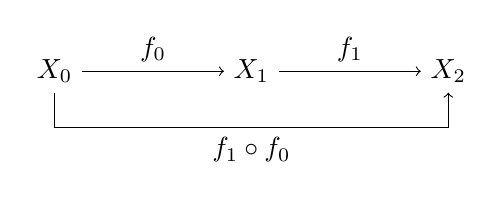
\begin{tikzpicture}[node distance=2.5cm, auto]
	\node (X) {$\bm{X_0}$};
	\node (Y) [right of=X] {$\bm{X_1}$};
	\node (n) [below of=Y,node distance=1cm] {$f_1 \circ f_0$};
	\node (Z) [right of=Y] {$\bm{X_2}$};
	\draw[->] (X) to node {$f_0$} (Y);
	\draw[->] (Y) to node {$f_1$} (Z);
%	\draw[->,bend right] (X) to node[swap] {$g \circ f$} (Z);
	\draw[->] (X) |- (n.90) -| (Z);\
\end{tikzpicture}
\end{figure}
	\end{enumerate}
\end{prop}
\begin{proof}
\begin{enumerate}
	\item Seja $A \in \topo$. Então $\id_X\inv(A)=A \in \topo$, logo $\id_x$ é contínua.
	
	\item Seja $A \in \topo_2$. Como $f_1$ é contínua, $f_1\inv(A) \in \topo_1$. Como $f_0$ é contínua, $f_0\inv(f_1\inv(A)) \in \topo_0$. Portanto
	\begin{equation*}
	(f_1 \circ f_0)\inv(A) = f_1\inv \circ f_0\inv (A) = f_0\inv(f_1\inv(A)) \in \topo_0.
	\end{equation*}
Logo $f_1 \circ f_0$ é contínua.
\end{enumerate}
\end{proof}

\section{Topologias Induzidas}

Nesta seção estudaremos como induzir topologias em conjuntos a partir de topologias que já temos. Isso será feito, em geral, de modo que uma ou mais funções sejam contínuas e a topologia induzida seja a menor ou a maior possível, dependendo do caso. Quando temos uma função de um conjunto em um espaço topológico, podemos induzir uma topologia nesse conjunto de modo que a topologia faça com  que a função seja contínua. Nesse caso, a maior topologia que faz a função ser contínua é a topologia discreta, e o nosso interesse será achar a menor topologia tal que a função é discreta. Quando temos uma função de um espaço topológico em um conjunto, o caso se inverte. A menor topologia tal que a função é contínua sempre é a topologia trivial, e o nosso interesse está na maior topologia que garante a continuidade. De maneira parecida, podemos induzir topologias garantindo a continuidade de várias funções e também considerando funções injetivas e sobrejetivas quado necessário. O estudo desta seção envolve a definição dessas noções e a investigação inicial como sobre esses objetos se comportam e por que são os menores ou maiores com determinadas características.

\subsection{Topologias Puxada e Inicial}

\begin{defi}
Sejam $X$ um conjunto, $\bm Y = (Y,\topo_Y)$ um espaço topológico e $f: X \to Y$ uma função. A \emph{topologia puxada} por $f$ de $\bm Y$ para $X$ é
	\begin{equation*}
	f^\star(\topo_Y) := \set{f^{-1}(A)}{A \in \topo_Y}.
	\end{equation*}
\end{defi}

\begin{prop}
Sejam $X$ um conjunto, $\bm Y = (Y,\topo_Y)$ um espaço topológico e $f: X \to Y$ uma função. Então $f^\star(\topo_Y)$, a topologia puxada por $f$ de $\bm Y$ para $X$, é uma topologia de $X$.
\end{prop}
\begin{proof}
(1) Notemos que, como $\emptyset \in \topo_Y$ e $\emptyset = f\inv(\emptyset)$, temos que $\emptyset \in f^\star(\topo_Y)$. (2) Seja $(A_i)_{i \in I}$ uma família de conjuntos em $f^\star(\topo_Y)$. Então, para cada $i \in I$, existe aberto $U_i \in \topo_Y$ tal que $A_i=f\inv(U_i)$. Como $\topo_Y$ é topologia, a união de abertos é aberto $\bigcup_{i \in I} U_i \in \topo_Y$. Portanto
	\begin{equation*}
	\bigcup_{i \in I} A_i = \bigcup_{i \in I} f\inv(U_i) = f\inv\left( \bigcup_{i \in I} U_i\right),
	\end{equation*}
logo $\bigcup_{i \in I} A_i \in f^\star(\topo_Y)$.
(3) Seja $(A_i)_{i=1}^n$ uma família de conjuntos em $f^\star(\topo_Y)$. Então, para cada $1 \leq i \leq n$, existe aberto $U_i \in \topo_Y$ tal que $A_i=f\inv(U_i)$. Como $\topo_Y$ é topologia, a interseção finita de abertos é aberto $\bigcap_{i=1}^n U_i \in \topo_Y$. Portanto
	\begin{equation*}
	\bigcap_{i=1}^n A_i = \bigcap_{i=1}^n f\inv(U_i) = f\inv\left( \bigcap_{i=1}^n U_i\right),
	\end{equation*}
logo $\bigcap_{i=1}^n A_i \in f^\star(\topo_Y)$.
\end{proof}

\begin{prop}
\label{topo:prop.cont.topo.pux}
Sejam $\bm X = (X,\topo_ X)$ e $\bm Y = (Y,\topo_ Y)$ espaços topológicos. Uma função $f: X \to Y$ é função contínua de $\bm X$ para $\bm Y$ se, e somente se, a topologia $f^\star(\topo_Y)$ puxada por $f$ de $\bm Y$ para $X$ é uma subtopologia de $\topo_ X$.
	\begin{equation*}
	f \in \cont(\bm X,\bm Y) \sse f^\star(\topo_Y) \subseteq \topo_X.
	\end{equation*}
\end{prop}
\begin{proof}
Suponha que $f \in \cont(\bm X,\bm Y)$ e seja $B \in f^\star(\topo_Y)$. Então existe $A \in \topo_Y$ tal que $B=f\inv(A)$. Como $f$ é contínua, segue que $f\inv(A) \in \topo_X$, portanto, $f^\star(\topo_Y) \subseteq \topo_X$. Reciprocamente, suponha que $f^\star(\topo_Y) \subseteq \topo_X$. Então, para todo $A \in \topo_Y$, $f\inv(A) \in f^\star(\topo_Y)$, portanto $f\inv(A) \in \topo_X$, o que mostra que $f \in \cont(\bm X,\bm Y)$.
\end{proof}

\begin{defi}
Sejam $\bm X$ um conjunto, $(\bm{X_i})_{i \in I} = (X_i,\topo_i)_{i \in I}$ uma família de espaços topológicos e, para todo $i \in I$, $f_i: X \to X_i$ uma função. A \emph{topologia inicial} de $X$ com respeito à família $(f_i)_{i \in I}$ é a menor topologia de $X$ tal que, para todo $i \in I$, $f_i$ é contínua.
\end{defi}

\begin{prop}
Sejam $\bm X$ um conjunto, $(\bm{X_i})_{i \in I} = (X_i,\topo_i)_{i \in I}$ uma família de espaços topológicos e, para todo $i \in I$, $f_i: X \to X_i$ uma função. A topologia inicial de $X$ com respeito à família $(f_i)_{i \in I}$ é a topologia
	\begin{equation*}
	\ger{\bigcup_{i \in I} {f_i}^\star(\topo_i)}.
	\end{equation*}
\end{prop}
\begin{proof}
Seja $\topo$ uma topologia de $X$ tal que, para todo $i \in I$, $f_i: X \to X_i$ é contínua. Então, para todo $i \in I$, ${f_i}^\star(\topo_i) \subseteq \topo$ (\ref{topo:prop.cont.topo.pux}), o que implica que $\bigcup_{i \in I} {f_i}^\star(\topo_i) \subseteq \topo$ e, portanto, $\ger{\bigcup_{i \in I} {f_i}^\star(\topo_i)} \subseteq \topo$.
\end{proof}

\subsection{Topologias Empurrada e Final}

\begin{defi}
Sejam $\bm X = (X,\topo_X)$ um espaço topológico, $Y$ um conjunto e $f: X \to Y$ uma função. A \emph{topologia empurrada} por $f$ de $\bm X$ para $Y$ é
	\begin{equation*}
	f_\star(\topo_X) := \set{A \subseteq Y}{f^{-1}(A) \in \topo_X}.
	\end{equation*}
\end{defi}

\begin{prop}
Sejam $\bm X = (X,\topo_X)$ um espaço topológico, $Y$ um conjunto e $f: X \to Y$ uma função. Então $\topo_Y := f_\star(\topo_X)$, a topologia empurrada por $f$ de $\bm X$ para $Y$, é uma topologia de $Y$.
\end{prop}
\begin{proof}
(1) Como $f\inv(\emptyset)=\emptyset$ e $f\inv(Y)=X$, segue que $\emptyset,Y \in f_\star(\topo_X)$. (2) Seja $(A_i)_{i \in I}$ uma família de conjuntos de $f_\star(\topo_X)$. Então, para cada $i \in I$, $f\inv(A_i) \in \topo_X$, o que implica que
\begin{equation*}
	f\inv \left( \bigcup_{i \in I} A_i \right) = \bigcup_{i \in I} f\inv(A_i) \in \topo_X,
	\end{equation*}
portanto $\bigcup_{i \in I} A_i \in f_\star(\topo_X)$. (3) Seja $(A_i)_{i=1}^n$ uma família de conjuntos de $f_\star(\topo_X)$. Então, para cada $1 \leq i \leq n$, $f\inv(A_i) \in \topo_X$, o que implica que
\begin{equation*}
	f\inv \left( \bigcap_{i=1}^n A_i \right) = \bigcap_{i=1}^n f\inv(A_i) \in \topo_X,
	\end{equation*}
portanto $\bigcap_{i=1}^n A_i \in f_\star(\topo_X)$.
\end{proof}

\begin{defi}
Sejam $\bm X$ um conjunto, $(\bm{X_i})_{i \in I} = (X_i,\topo_i)_{i \in I}$ uma família de espaços topológicos e, para todo $i \in I$, $f_i: X_i \to X$ uma função. A \emph{topologia final} de $X$ com respeito à família $(f_i)_{i \in I}$ é a maior topologia de $X$ tal que, para todo $i \in I$, $f_i$ é contínua.
\end{defi}

\begin{prop}
Sejam $\bm X$ um conjunto, $(\bm{X_i})_{i \in I} = (X_i,\topo_i)_{i \in I}$ uma família de espaços topológicos e, para todo $i \in I$, $f_i: X_i \to X$ uma função. A topologia final de $X$ com respeito à família $(f_i)_{i \in I}$ é a topologia
	\begin{equation*}
	\bigcap_{i \in I} {f_i}_\star(\topo_i).
	\end{equation*}
\end{prop}
\begin{proof}
Seja $\topo$ uma topologia de $X$ tal que, para todo $i \in I$, $f_i: X_i \to X$ é contínua, e seja $A \in \topo$. Então, para todo $i \in I$, $f_i \inv(A) \in \topo_i$, o que implica que $A \in {f_i}_\star(\topo_i)$, portanto $A \in \bigcap_{i \in I} {f_i}_\star(\topo_i)$. Isso mostra que $\topo \subseteq \bigcap_{i \in I} {f_i}_\star(\topo_i)$, e como interseção de topologiaas é topologia, segue o procurado.
\end{proof}

\subsection{Produto de Espaços Topológicos}

\begin{defi}
Seja $(\bm{X_i})_{i \in I} = (X_i,\topo_i)_{i \in I}$ uma família de espaços topológicos. O \emph{produto} da família $(\bm{X_i})_{i \in I}$ é o par
	\begin{equation*}
	\prod_{i \in I} \bm{X_i} := \left( \prod_{i \in I} X_i , \ger{\bigcup_{i \in I}{\pi_i}^\star(\topo_i)} \right).
	\end{equation*}
A topologia $\ger{\bigcup_{i \in I}{\pi_i}^\star(\topo_i)}$ é a \emph{topologia produto} de $\prod_{i \in I} X_i$.
\end{defi}

\begin{prop}
Sejam $(\bm{X_i})_{i \in I} = (X_i,\topo_i)_{i \in I}$ uma família de espaços topológicos e $X = \prod_{i \in I} X_i$ o produto de conjuntos. A topologia produto de $X$ é a topologia gerada pela base cujos elementos são $\prod_{i \in I} A_i$, tal que $A_i \in \topo_i$ e existe $J \subseteq I$ finito com $A_i = X_i$ para $i \in I \setminus J$.
\end{prop}
\begin{proof}
Como $\pi_i = \pi_i \circ \id_X$, segue de uma propriedades básica de imagem inversa de produto (\ref{conj:prop.im.inv.prod}) que
	\begin{equation*}
	\prod_{i \in I} A_i = \id_X\inv \left(\prod_{i \in I} A_i\right) = \bigcap_{i \in I} \pi_i\inv(A_i)
	\end{equation*}
Para todo $i \in I \setminus J$, $A_i=X_i$, então $\pi_i\inv(A_i)=X$ e, portanto,
	\begin{equation*}
	\bigcap_{i \in I\setminus J} \pi_i\inv(A_i) = \bigcap_{i \in I\setminus J} X = X.
	\end{equation*}
Isso implica que
	\begin{equation*}
	\bigcap_{i \in I} \pi_i\inv(A_i) = \left(\bigcap_{i \in I\setminus J} \pi_i\inv(A_i)\right) \cap \left(\bigcap_{j \in J} \pi_j\inv(A_j)\right) =  \bigcap_{j \in J} \pi_j\inv(A_j)
	\end{equation*}
Logo $\prod_{i \in I} A_i = \bigcap_{j \in J} \pi_j\inv(A_j)$. Seja $A$ aberto da topologia descrita na proposição. Então
	\begin{equation*}
	A = \bigcup_{k \in K} A_k = \bigcup_{k \in K}\prod_{i \in I} A_{ki} = \bigcup_{k \in K}\bigcap_{j \in J} \pi_j\inv (A_{kj}),
	\end{equation*}
o que mostra que $A$ é aberto da topologia produto. O resto da demonstração é simples.
\end{proof}

\begin{prop}[Propriedade Universal]
Sejam $(\bm{X_i})_{i \in I} = (X_i,\topo_i)_{i \in I}$ uma família de espaços topológicos, $\bm T = (T,\topo_T)$ um espaço topológico e, para todo $i \in I$, $f_i: \bm T \to \bm{X_i}$ uma função contínua. Então existe uma única função contínua $f: \bm T \to \prod_{i \in I} \bm{X_i}$ tal que, para todo $i \in I$, $\pi_i \circ f = f_i$ (o diagrama comuta).
\begin{figure}
\centering
\begin{tikzpicture}[node distance=2.5cm, auto]
	\node (P) {$\displaystyle\prod_{i \in I} \bm{X_i}$};
	\node (Ci) [below of=P] {$\bm{X_i}$};
	\node (X) [left of=Ci] {$\bm{T}$};
	\draw[->] (X) to node [swap] {$f_i$} (Ci);
	\draw[->, dashed] (X) to node {$f$} (P);
	\draw[->] (P) to node {$\pi_i$} (Ci);
\end{tikzpicture}
\end{figure}
\end{prop}
\begin{defi}
Defina a função
	\begin{align*}
	\func{f}{T}{ \prod_{i \in I} X_i}{ x}{ (f_i(x))_{i \in I}}.
	\end{align*}
Pela propriedade universal do produto de conjuntos, $f$ é única e $\pi_i \circ f = f_i$. Resta mostrar que $f$ é contínua. Seja $A \in \topo_X$. Então $A=\bigcup_{k \in K} A_k$ é uma união de abertos básicos $A_k \in \topo$. Isso significa que, para todo $k \in K$, $A_k = \prod_{i \in I} A_{ki}$, com $A_{ki} \in \topo_i$ para todo $i \in I$ e existe $J_k \subseteq I$ finito tal que, para todo $i \in I \setminus J_k$, $A_{ki} = X_i$. Assim, por propriedades básicas de imagem inversa de união e produto (\ref{conj:prop.im.inv.prod}),
		\begin{equation*}
		f\inv(A) = f\inv\left(\bigcup_{k \in K}\prod_{i \in I} A_{ki}\right) = \bigcup_{k \in K} f\inv \left( \prod_{i \in I} A_{ki} \right) = \bigcup_{k \in K}\bigcap_{i \in I}f_i\inv(A_{ki}).
		\end{equation*}
Seja $k \in K$. Como, para todo $i \in I \setminus J_k$, $A_{ki} = X_i$, então $f_i\inv(A_{ki}) = f_i\inv(X_i) = T$. Disso segue que
	\begin{equation*}
	\bigcap_{i \in I}f_i\inv(A_{ki}) = \bigcap_{j \in J_k}f_j\inv(A_{kj})
	\end{equation*}
e, portanto,
	\begin{equation*}
	f\inv(A) = \bigcup_{k \in K}\bigcap_{j \in J_k}f_j\inv(A_{kj}).
	\end{equation*}
Seja $k \in K$. Para todo $j \in J_k$, $f_j$ é contínua, o que impica que $f_j\inv(A_{kj})$ é aberto e, por $J_k$ ser finito, a interseção $\bigcap_{j \in J_k}f_j\inv(A_{kj})$ é aberta. Isso significa que a união $\bigcup_{k \in K}\bigcap_{j \in J_k}f_j\inv(A_{kj})$ é aberta e, portanto, $f\inv(A) \in \topo_T$. Logo $f$ é contínua.
\end{defi}

\subsection{Coproduto de Espaços Topológicos}

\begin{defi}
Seja $(\bm{X_i})_{i \in I} = (X_i,\topo_i)_{i \in I}$ uma família de espaços topológicos. O \emph{coproduto} da família $(\bm{X_i})_{i \in I}$ é o par
	\begin{equation*}
	\coprod_{i \in I} \bm{X_i} := \left( \coprod_{i \in I} X_i , \bigcap_{i \in I}{\iota_i}_\star(\topo_i) \right).
	\end{equation*}
A topologia $\bigcap_{i \in I}{\pi_i}_\star(\topo_i)$ é a \emph{topologia coproduto} de $\coprod_{i \in I} X_i$.
\end{defi}

\begin{prop}[Propriedade Universal]
Sejam $(\bm{X_i})_{i \in I} = (X_i,\topo_i)_{i \in I}$ uma família de espaços topológicos, $\bm T = (T,\topo_T)$ um espaço topológico e, para todo $i \in I$, $f_i: \bm{X_i} \to \bm T$ uma função contínua. Então existe uma única função contínua $f: \coprod_{i \in I} \bm{X_i} \to \bm T$ tal que, para todo $i \in I$, $f \circ \iota_i = f_i$ (o diagrama comuta).
\begin{figure}
\centering
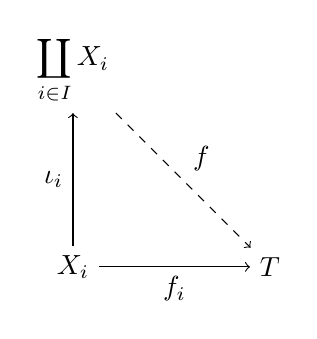
\begin{tikzpicture}[node distance=2.5cm, auto]
	\node (Ci) {$\bm{X_i}$};
	\node (S) [above of=Ci] {$\displaystyle\coprod_{i \in I} \bm{X_i}$};
	\node (X) [right of=Ci] {$\bm T$};
	\draw[->] (Ci) to node [swap] {$f_i$} (X);
	\draw[->, dashed] (S) to node {$f$} (X);
	\draw[->] (Ci) to node {$\iota_i$} (S);
\end{tikzpicture}
\end{figure}
\end{prop}

\subsection{Subespaços Topológicos}

\begin{defi}
Sejam $(X,\topo)$ um espaço topológico e $S \subseteq X$ um subconjunto. A \emph{topologia induzida} por $\topo$ em $S$ é o conjunto
	\begin{equation*}
	\topo|_S := \set{A \cap S}{A \in \topo}.
	\end{equation*}
\end{defi}

\begin{prop}
Sejam $(X,\topo)$ um espaço topológico e $S \subseteq X$ um subconjunto. A topologia induzida por $\topo$ em $S$ é o conjunto
	\begin{equation*}
	\topo|_S = \iota_\star(\topo),
	\end{equation*}
a maior topologia tal que a inclusão $\iota: S \to X$ é contínua.
\end{prop}

\begin{prop}
Sejam $(X,\topo)$ um espaço topológico e $S \subseteq X$ um subconjunto. A topologia induzida por $\topo$ em $S$ é uma topologia de $S$.
\end{prop}
\begin{proof}
(1) Notemos que $\emptyset,Y \in \topo|_Y$, pois $\emptyset \cap Y = \emptyset$ e $X \cap Y = Y$. (2) Seja $(A_i)_{i \in I}$ uma família de abertos de $\topo|_Y$. Então, para cada $i \in I$, existe um aberto $B_i \in \topo$ tal que $A_i = B_i \cap Y$. Assim, temos que
	\begin{equation*}
	\bigcup_{i \in I} A_i = \bigcup_{i \in I} (B_i \cap Y) = \left( \bigcup_{i \in I} B_i \right) \cap Y,
	\end{equation*}
que pertence à topologia induzida pois $\bigcup_{i \in I} B_i \in \topo$. (3) Seja $(A_i)_{i=1}^n$ uma família de abertos de $\topo|_Y$. Então, para cada $1 leq i leq n$, existe um aberto $B_i \in \topo$ tal que $A_i = B_i \cap Y$. Assim, temos que
	\begin{equation*}
	\bigcap_{i=1}^n A_i = \bigcap_{i=1}^n (B_i \cap Y) = \left( \bigcap_{i=1}^n B_i \right) \cap Y,
	\end{equation*}
que pertence à topologia induzida pois $\bigcap_{i=1}^n B_i \in \topo$.
\end{proof}

\begin{prop}[Propriedade característica]
Sejam $\bm X=(X,\topo_X)$ e $(Y,\topo_Y)$ espaços topológicos e $\bm S \subseteq \bm X$ um subespaço. Uma função $f: Y \to S$ é contínua se, e somente se, $\iota \circ f: Y \to X$ é contínua (o diagrama comuta).
\begin{figure}
\centering
\begin{tikzpicture}[node distance=2.5cm, auto]
	\node (X) {$\bm X$};
	\node (S) [below of=X] {$\bm S$};
	\node (Y) [left of=S] {$\bm{T}$};
	\draw[->] (Y) to node [swap] {$f$} (S);
	\draw[->] (Y) to node {$\iota \circ f$} (X);
	\draw[->] (S) to node [swap] {$\iota$} (X);
\end{tikzpicture}
\end{figure}
\end{prop}

\paragraph*{Proposição} Restrição de função contínua é contínua na topologia induzida.

\begin{prop}[Colagem por abertos]
Sejam $\bm X$ e $\bm Y$ espaços topológicos, $f: X \to Y$ uma função e $(X_i)_{i \in I}$ uma cobertura de $X$ por conjuntos abertos tal que, para todo $i \in I$, $f|_{X_i}: X_i \to Y$ é contínua. Então $f: X \to Y$ é contínua.
\end{prop}

\begin{prop}[Colagem por fechados]
Sejam $\bm X$ e $\bm Y$ espaços topológicos, $f: X \to Y$ uma função e $(X_i)_{i=1}^n$ uma cobertura de $X$ por conjuntos fechados tal que, para todo $1 \leq i \leq n$, $f|_{X_i}: X_i \to Y$ é contínua. Então $f: X \to Y$ é contínua.
\end{prop}

\subsection{Quociente de Espaços Topológicos}

\begin{defi}
Sejam $\bm X = (X,\topo)$ um espaço topológico e $\sim$ uma relação de equivalência em $X$. O \emph{espaço quociente} com respeito a $\sim$ é o espaço topológico
	\begin{equation*}
	\bm{\quo{X}{\sim}} := \left( \quo{X}{\sim}, \pi^\star(\topo) \right),
	\end{equation*}
em que $\pi: X \to \quo{X}{\sim}$ é a projeção canônica de equivalências.
\end{defi}

É fácil notar que os abertos de $\bm{\quo{X}{\sim}}$ são conjuntos de classes de equivalência cuja união é um aberto de $\bm X$. Notemos, ainda, que se $f: X \to Y$ é sobrejetivo, existe uma relação de equivalência em $X$ induzida por $f$, definida como dois elementos são equivalentes se suas imagens são iguais, e essa relação de equivalência faz com que possamos identificar $Y$ com $\quo{X}{\sim}$ como conjuntos. Definimos a topologia em $Y$ de modo que $Y$ e $\quo{X}{\sim}$ sejam homeomorfos.

\begin{prop}[Propriedade característica]
Sejam $\bm X=(X,\topo_X)$ e $(Y,\topo_Y)$ espaços topológicos e $\bm Q$ um espaço quociente de $\bm X$. Uma função $f: Q \to Y$ é contínua se, e somente se, $f \circ \pi: X \to Y$ é contínua (o diagrama comuta).
\begin{figure}
\centering
\begin{tikzpicture}[node distance=2.5cm, auto]
	\node (Q) {$\bm Q$};
	\node (X) [above of=Q] {$\bm X$};
	\node (Y) [right of=Q] {$\bm Y$};
	\draw[->] (Q) to node [swap] {$f$} (Y);
	\draw[->] (X) to node {$f \circ \pi$} (Y);
	\draw[->] (X) to node [swap] {$\pi$} (Q);
\end{tikzpicture}
\end{figure}
\end{prop}


\chapter{Axiomas de Separação}

\section{Noções de Separação de Conjuntos}

Nesta seção são apresentadas algumas noções de como dois conjuntos de um espaço topológico podem ser separadas. As duas noções mas simples de separação são noções conjuntistas. A primeira é a de conjuntos distintos, ou diferentes, $A \neq B$, e a outra é a de conjuntos disjuntos, $A \cap B = \emptyset$. A seguir, mostramos noções que envolvem construções topológicas e não meramente conjuntistas.

\begin{defi}
Sejam $\bm X$ um espaço topológico e $A,B \subseteq X$. Definimos as seguintes relações entre $A$ e $B$:
	\begin{enumerate}
	\item (\emph{Separação}). Cada conjunto é disjunto do feixo do outro.
	\begin{equation*}
	A \cap \fec{B} = \fec{A} \cap B = \emptyset.
	\end{equation*}
	\item (\emph{Separação por vizinhanças}). Existem vizinhanças $V_A \in \viz_A$ e $V_B \in \viz_B$ que são disjuntas.
	\begin{equation*}
	V_A \cap V_B = \emptyset.
	\end{equation*}
	\item (\emph{Separação por função contínua}). Existe uma função contínua $f \in \cont(X,[0,1])$ tal que
	\begin{equation*}
	f(A)=\{0\} \e f(B)=\{1\}.
	\end{equation*}
	\item (\emph{Separação precisa por função contínua}). Existe uma função contínua $f \in \cont(X,[0,1])$ tal que
	\begin{equation*}
	f\inv(\{0\})=A \e f\inv(\{1\})=B.
	\end{equation*}
	\end{enumerate}
Cada uma das relações vale entre pontos $x,y \in X$, ou entre um conjunto $A$ e um ponto $x$, ao considerarmos no lugar no ponto o conjunto unitário que o contém: valem entre os conjuntos $\{x\}$ e $\{y\}$, ou entre $A$ e $\{x\}$, respectivamente.
\end{defi}

	As primeiras duas relações binárias são claramente simétricas, mas isso não é necessariamente claro no caso da terceira e quarta. No entanto, isso pode ser concluído ao cosiderar, dada uma função $f$ que faz $A$ e $B$ separados por função contínua, a função $1-f$ que faz o mesmo entre $B$ e $A$.

\begin{prop}
Sejam $\bm X$ um espaço topológico e $A,B \subseteq X$. Então
	\begin{enumerate}
	\item Se $A$ e $B$ são precisamente separados por função contínua, então são separados por função contínua.
	\item Se $A$ e $B$ são separados por função contínua, então são separados por vizinhanças.
	\item Se $A$ e $B$ são separados por vizinhanças, então são separados.
	\item Se $A$ e $B$ são separados, então são disjuntos.
	\end{enumerate}
\end{prop}

% DÚVIDA: As relações de separação negadas são relações de equivalência? Pois indintinguibilidade topológica é, e ela é a negação de separação de pontos (não exatamente). Tentar entender melhor isso.


\section{Espaços Distinguíveis}

\begin{defi}
Seja $\bm X$ um espaço topológico. Pontos \emph{topologicamente indisntinguíveis em $\bm X$} são pontos $x,y \in X$ tais que $\viz_x = \viz_y$. Pontos \emph{topologicamente disntinguíveis em $\bm X$} são pontos que não são topologicamente indistinguíveis.
\end{defi}

\begin{prop}
Seja $\bm X$ um espaço topológico. A relação binária de indistinguibilidade topológica é uma relação de equivalência em $X$.
\end{prop}
\begin{proof}
Denotemos por $\sim$ a relação binária de indistinguibilidade topológica. Sejam $x,y,z \in X$. Para mostrar a reflexividade, notemos que, como $\viz_x=\viz_y$, então $x \sim x$. Para mostrar a simetria, se $x \sim y$, então $\viz_x=\viz_y$, o que é equivalente a $\viz_y=\viz_x$ e, portanto, $y \sim x$. Por fim, para mostrar a transitividade, se $x \sim y$ e $y \sim z$, então $\viz_x=\viz_y$ e $\viz_y=\viz_z$, o que implica $\viz_x=\viz_z$ e, portanto, $x \sim z$.
\end{proof}

O fato de que essa é uma relação de equivalência mostra que podemos obter a partir de qualquer espaço topológico um espaço topológico em que nenhum ponto é topologicamente indisntinguível. Para isso, basta considerar o espaço quociente definido pela relação. de indistinguibilidade topológica. Espaços com essa propriedade são definidos a seguir.

\begin{defi}[$T_0$]
Um espaço topológico \emph{distinguível} é um espaço topológico $\bm X$ em que todo par de pontos distintos é topologicamente distinguível:
	\begin{equation*}
	\forall x,y \in X \quad x \neq y \quad \Rightarrow \quad \viz_x \neq \viz_y.
	\end{equation*}
\end{defi}

\begin{prop}
Seja $\bm X$ um espaço topológico. São equivalentes as seguites propriedades:
	\begin{enumerate}
	\item $\bm X$ é dinstinguível.
	\item $\forall x,y \in X \quad x \neq y \quad \Rightarrow \quad \viz_x \nsubseteq \viz_y \ou \viz_y \nsubseteq \viz_x$.
	\item $\forall x,y \in X \quad x \neq y \quad \Rightarrow \quad x \notin \fec{\{y\}} \ou y \notin \fec{\{x\}}$.
	\item $\forall x,y \in X \quad x \neq y \quad \Rightarrow \quad \fec{\{x\}} \neq \fec{\{y\}}$.	
\end{enumerate}
\end{prop}

\begin{prop}
Sejam $\bm X$ um espaço topológico distinguível e $Y \subseteq X$. Então $\bm Y$ é um espaço topológico distinguível.
\end{prop}

\begin{prop}
Seja $(X_i)_{i \in I}$ uma família não vazia de espaços topológicos não vazios. O espaço produto $\bm{\bigtimes X_i}$ é distinguível se, e somente se, todos os espaços $\bm X_i$ são distinguíveis.
\end{prop}

\section{Espaços Acessíveis}

\begin{defi}[$T_1$]
Um espaço topológico \emph{acessível} é um espaço topológico $\bm X$ em que
	\begin{equation*}
	\forall x,y \in X \quad x \neq y \quad \Rightarrow \quad \viz_x \nsubseteq \viz_y \e \viz_y \nsubseteq \viz_x.
	\end{equation*}
\end{defi}

\begin{prop}[$T_1 \Rightarrow T_0$]
Seja $\bm X$ um espaço topológico. Se $\bm X$ é acessível, então $\bm X$ é dintinguível.
\end{prop}
\begin{proof}
Se $\bm X$ é acessível, então, para todos $x,y \in X$ tais que $x \neq y$, temos que $\viz_x \nsubseteq \viz_y \e \viz_y \nsubseteq \viz_x$. Mas isso implica que $\viz_x \nsubseteq \viz_y \ou \viz_y \nsubseteq \viz_x$, o que é equivalente a $\viz_x \neq \viz_y$. Logo $\bm X$ é dintinguível.
\end{proof}

\begin{prop}
Seja $\bm X$ um espaço topológico. São equivalentes as seguintes propriedades:
	\begin{enumerate}
	\item $\bm X$ é acessível.
	\item Todo par de pontos distintos é separado:
		\begin{equation*}
		\forall x,y \in X \quad x \neq y \quad \Rightarrow \quad x \notin \fec{\{y\}} \e y \notin \fec{\{x\}}.
		\end{equation*}
	\item $\forall x,y \in X \quad x \neq y \quad \Rightarrow \quad \exists U \in \viz_x,\ V \in \viz_y \qquad y \notin U \e x \notin V$.
	\item $\forall x \in X \quad \fec{\{x\}}=\{x\}$.
	\end{enumerate}
\end{prop}

\begin{prop}
Sejam $\bm X$ um espaço topológico acessível e  $Y \subseteq X$. Então $\bm Y$ é um espaço topológico acessível.
\end{prop}

\begin{prop}
Seja $(X_i)_{i \in I}$ uma família não vazia de espaços topológicos não vazios. O espaço produto $\bm{\bigtimes X_i}$ é acessível se, e somente se, todos os espaços $\bm X_i$ são acessíveis.
\end{prop}

\section{Espaços Separados}

\begin{defi}[$T_2$]
Um espaço topológico \emph{separado} é um espaço topológico $\bm X$ em que todo par de pontos distintos é separado por vizinhanças:
	\begin{equation*}
	\forall x,y \in X \quad x \neq y \quad \Rightarrow \quad \exists U \in \viz_x,\ V \in \viz_y \quad U \cap V = \emptyset.
	\end{equation*}
\end{defi}
Esses espaços também são conhecidos como espaços de Hausdorff.

\begin{prop}[$T_2 \Rightarrow T_1$]
Seja $\bm X$ um espaço topológico. Se $\bm X$ é separado, então $\bm X$ é acessível.
\end{prop}

\begin{prop}
Seja $\bm X$ um espaço topológico. São equivalentes as seguintes propriedades:
	\begin{enumerate}
	\item $\bm X$ é separado.
	\item Toda rede convergente em $\bm X$ tem limite único.
	\item Todo filtro convergente em $\bm X$ tem limite único.
	\end{enumerate}
\end{prop}

\begin{prop}
Sejam $\bm X$ um espaço topológico separado e $Y \subseteq X$. Então $\bm Y$ é um espaço topológico separado.
\end{prop}

\begin{prop}
Seja $(X_i)_{i \in I}$ uma família não vazia de espaços topológicos não vazios. O espaço produto $\bm{\bigtimes X_i}$ é separado se, e somente se, todos os espaços $\bm X_i$ são separados.
\end{prop}

\begin{prop}
Sejam $\bm X$ um espaço topológico, $\bm Y$ um espaço topológico separado, $D \subseteq X$ um subconjunto denso em $X$ e $f,g: X \to Y$ funções contínuas tais que $f|_D=g|_D$. Então $f=g$.
\end{prop}

\section{Espaços Regulares}

\begin{defi}
Um espaço topológico \emph{regular} é um espaço topológico
% $\bm X$
em que é possível separar por vizinhanças qualquer ponto de qualquer conjunto fechado que não o contém.
%: para todo $x \in X$ e para todo conjunto fechado $F \subseteq X$,
%	\begin{equation*}
%	F \cap \{x\}=\emptyset \quad \Rightarrow \quad \exists U \in \viz_x, \exists V \in \viz_F \quad U \cap V = \emptyset.
%	\end{equation*}
\end{defi}

Espaços seprados regulares são também chamados de $T_3$.

\begin{prop}
Seja $\bm X$ um espaço topológico regular. Então $\bm X$ é separado se, e somente se, é distinguível.
\end{prop}
\begin{proof}
Sabemos que todo espaço separado é distinguível. Para demonstrar a recíproca, supondo que $\bm X$ é distinguível, então para todos pontos $x,y \in X$, $x \notin \fec{\{y\}}$ ou $y \notin \fec{\{x\}}$. Sem perda de generalidade, assumamos o primeiro caso. Seja $F := \fec{\{y\}}$. Então $F$ é fechado e $x \notin F$. Da regularidade de $\bm X$, segue que existem $U \in \viz_x$ e $V \in \viz_{F}$ tais que $U \cap V = \emptyset$. Como $y \in F$, então $V \in \viz_y$, o que implica que $\bm X$ é separado.
\end{proof}

\begin{prop}
Seja $\bm X$ um espaço topológico. São equivalentes as seguintes propriedades:
	\begin{enumerate}
	\item $\bm X$ é regular.
	\item Para todos ponto $x \in X$ e aberto $A \in \viz_x$, existe aberto $V \in \viz_x$ tal que
		\begin{equation*}
		x \in V \subseteq \fec{V} \subseteq A.
		\end{equation*}
	\end{enumerate}
\end{prop}

\begin{prop}
Sejam $\bm X$ um espaço topológico regular e $Y \subseteq X$. Então $\bm Y$ é um espaço topológico regular.
\end{prop}

\begin{prop}
Seja $(X_i)_{i \in I}$ uma família não vazia de espaços topológicos não vazios. O espaço produto $\bm{\bigtimes X_i}$ é regular se, e somente se, todos os espaços $\bm X_i$ são regulares.
\end{prop}

\section{Espaços Completamente Regulares}

\begin{defi}
Um espaço topológico \emph{completamente regular} é um espaço topológico
% $\bm X$
em que é possível separar por função contínua qualquer ponto de qualquer conjunto fechado que não o contém.
%: para todo $x \in X$ e para todo conjunto fechado $F \subseteq X$,
%	\begin{equation*}
%	\{x\} \cap F=\emptyset \quad \Rightarrow \quad \exists f \in \mathcal{C}(X,[0,1]) \quad f(x)=\{0\} \e f(F)=\{1\}.
%	\end{equation*}
\end{defi}

\begin{prop}
Seja $\bm X$ um espaço topológico. Se $\bm X$ é completamente regular, então $\bm X$ é regular.
\end{prop}

\begin{prop}
Sejam $\bm X$ um espaço topológico completamente regular e $Y \subseteq X$. Então $\bm Y$ é um espaço topológico completamente regular.
\end{prop}

\begin{prop}
Seja $(X_i)_{i \in I}$ uma família não vazia de espaços topológicos não vazios. O espaço produto $\bm{\bigtimes X_i}$ é completamente regular se, e somente se, todos os espaços $\bm X_i$ são completamente regulares.
\end{prop}

\section{Espaços Normais}

\begin{defi}
Um espaço topológico \emph{normal} é um espaço topológico
% $\bm X$ 
em que todo par de conjuntos fechados disjuntos é separado por vizinhanças.
% : para todos fechados $F,G \subseteq X$,
%	\begin{equation*}
%	F \cap G = \emptyset \quad \Rightarrow \quad \exists U \in \viz_F,\ V \in \viz_G \quad U \cap V = \emptyset.
%	\end{equation*}
\end{defi}

Espaços separados normais são também chamados de $T_4$.

\begin{prop}
Seja $\bm X$ um espaço topológico normal. Então $\bm X$ é separado se, e somente se, é acessível.
\end{prop}
\begin{proof}
Sabemos que todo espaço separado é distinguível. Para demonstrar a recíproca, suponhamos que $\bm X$ é acessível e sejam $x,y \in X$ tais que $x \neq y$. Então vale que $\fec{\{x\}}=\{x\}$ e $\fec{\{y\}}=\{y\}$. Como $x \neq y$, da normalidade de $\bm X$ existem $V_x \in \viz_x$ e $V_y \in \viz_y$ tais que $V_x \cap V_y = \emptyset$; ou seja, $\bm X$ é separado.
\end{proof}

\begin{prop}
Seja $\bm X$ um espaço topológico. São equivalentes as seguintes propriedades:
	\begin{enumerate}
	\item $\bm X$ é normal.
	\item Para todos fechado $F$ e aberto $A \in \viz_F$, existe aberto $V \in \viz_F$ tal que
		\begin{equation*}
		F \subseteq V \subseteq \fec{V} \subseteq A.
		\end{equation*}
	\end{enumerate}
\end{prop}

\begin{prop}
Sejam $\bm X$ um espaço topológico normal e $Y \subseteq X$ fechado. Então $\bm Y$ é um espaço topológico normal.
\end{prop}


\begin{prop}[Lema de Urysohn]
Um espaço topológico $\bm X$ é normal se, e somente se, todo par de conjuntos fechados é separado por função contínua.
% : para todos conjuntos fechados $F,G \subseteq X$,
%	\begin{equation*}
%	F \cap G = \emptyset \quad \Rightarrow \quad \exists f \in \mathcal{C}(X,[0,1]) \quad f(F)=\{0\} \e f(G)=\{1\}.
%	\end{equation*}
\end{prop}
\begin{proof}
Primeiro, suponhamos que existe função contínua $f:X \to [0,1]$ tal que $f(F)= \{0\}$ e $f(G)=\{1\}$. Definamos $U := f^{-1}(\left[0,\frac{1}{2}\right))$ e $V := f^{-1}((\frac{1}{2},1))$. Como $f$ é contínua, $U$ e $V$ são abertos. Ainda, $F \subseteq U$ e $G \subseteq V$. Por fim, como $U \cap V = \emptyset$, concluímos que $\bm X$ é normal.

Para demonstrar a recíproca, suponhamos que $\bm X$ é normal. Sejam $F,G \subseteq X$ conjuntos fechados disjuntos. Como $G^\complement$ é aberto e $F \subseteq G^\complement$, existe aberto $A_{\frac{1}{2}}$ tal que $F \subseteq A_{\frac{1}{2}} \subseteq \fec{A_{\frac{1}{2}}} \subseteq G^\complement$. Logo existem abertos $A_{\frac{1}{4}}$ e $A_{\frac{3}{4}}$ tais que
	\begin{equation*}
	F \subseteq A_{\frac{1}{4}} \subseteq \fec{A_{\frac{1}{4}}} \subseteq A_{\frac{1}{2}} \subseteq \fec{A_{\frac{1}{2}}} \subseteq A_{\frac{3}{4}} \subseteq \fec{A_{\frac{3}{4}}} \subseteq G^\complement.
	\end{equation*}
Seja $D := \{\frac{k}{2^n}:n \in \N^* \e k \in \{1,\ldots,2^n-1\}\}$. Indutivamente obtemos, para cada $r \in D$, um aberto $A_r$ tal que
	\begin{equation*}
	F \subseteq A_{\frac{1}{2^n}} \subseteq \fec{A_{\frac{1}{2^n}}} \subseteq A_{\frac{2}{2^n}} \subseteq \fec{A_{\frac{2}{2^n}}}\subseteq \cdots \subseteq A_{\frac{2^n-1}{2^n}} \subseteq \fec{A_{\frac{2^n-1}{2^n}}} \subseteq G^\complement.
	\end{equation*}
	
	...
	
	...
\end{proof}

















\chapter{Invariantes Topológicos}

\section{Conexidade}

Definimos o conceito de desconexo antes por ele ser mais intuitivo de ser enunciado. Ser desconexo é ter como separar o espaço $\bm X$ em dois conjuntos disjuntos, aberto e não triviais (não são $\emptyset$ nem $X$). Esses abertos cobrem todo espaço e, como são abertos, o separam pela definição de separação de conjuntos.

\begin{defi}
Um espaço topológico \emph{desconexo} é um espaço topológico $\bm X$ tal que $X$ admite partição por dois conjuntos abertos. Um espaço topológico \emph{conexo} é um espaço topológico que não é desconexo. Um subconjunto de $X$ é conexo ou desconexo de acordo com sua topologia induzida.
\end{defi}

Uma partição por dois abertos é equivalente a uma cobertura por dois conjuntos abertos, disjuntos e não triviais. Notemos que, por essa definição, o espaço topológico $\bm \emptyset$ é conexo, pois todos subconjuntos de $\emptyset$ são triviais, logo $\emptyset$ não admite partições. A conexidade de $\emptyset$ não é consenso entre autores, mas adotaremos esse resultado aqui. É importante notar que, na definição, porderíamos escolher uma partição por conjuntos fechados, já que, como cada conjunto da partição é o complementar do outro, ambos são fechados, pois ambos são abertos. A definição de separação de conjuntos vale nesse caso, os conjuntos da partição são separados no sentido que cada um é disjunto do fecho do outro, já que são fechados e disjuntos. Isso sugere que conexidade está relacionada com o problema de confusão semântica clássica em topologia: nem todo conjunto aberto é necessariamente não fechado, e vice-versa. Claro que $\emptyset$ e $X$ são sempre abertos e fechados, mas em espaços conexos eles são os únicos. Com o conceito de conexidade, temos o seguinte resultado.

\begin{prop}
Um espaço topológico $\bm X$ é conexo se, e somente se, não existe um conjunto não trivial que é aberto e fechado.
\end{prop}
\begin{proof}
Vamos mostrar a ida e a volta pela contrapositiva. Se $\bm X$ é desconexo, os conjuntos que formam sua partição por abertos são ambos abertos e fechados. Reciprocamente, se $A \subseteq X$ é não tricial, aberto e fechado, $A^\complement$ também é não trivial e aberto (e fechado), logo $\{A, A^\complement\}$ é uma partição de $X$ por dois conjuntos abertos.
\end{proof}

As noções de conexidade de um espaço topológico e de um subconjunto de um espaço topológico são, de fato, a mesma, mas alguns cuidados devem ser tomados para escolher onde os conjuntos são abertos ou fechados, se na topologia original ou na induzida. A proposição a seguir oferece um critério para conjuntos conexos.

\begin{prop}
Seja $\bm X$ um espaço topológico. Então $S \subseteq X$ é conexo se, e somente se, não existem conjuntos não triviais separados em $\bm X$ cuja união é $S$.
\end{prop}
\begin{proof}
Se $S$ é desconexo, existe uma partição $\{A,B\}$ de $S$ por abertos de $\bm S$. Então $A \cup B=S$,
	\begin{equation*}
	A \cap \fec{B}^{_X} = (A \cap S) \cap \fec{B}^{_X} = A \cap (S \cap \fec{B}^{_X}) = A \cap \fec{B}^{_S} = A \cap B = \emptyset
	\end{equation*}
e, similamente, $\fec{A}^{_X} \cap B = \emptyset$, o que mostra que $A$ e $B$ são separados em $\bm X$. Reciprocamente, se existem $A,B \subseteq X$ conjuntos não triviais separados em $\bm X$ tais que $A \cup B=S$, então
	\begin{equation*}
	\fec{A}^{_S} = S \cap \fec{A}^{_X} = (A \cap B) \cap \fec{A}^{_X} = (A \cap \fec{A}^{_X}) \cup (B \cap \fec{A}^{_X}) = A \cup \emptyset = A
	\end{equation*}
e, similarmente, $\fec{B}^{_S}=B$, portanto $\{A,B\}$ é partição de $S$ por fechados de $\bm S$, o que mostra que $\bm S$ é desconexo.
\end{proof}

A seguir, enunciamos uma equivalência da definição de conexidade e um resultado trivial, mas importantíssimo na topologia: conexidade é um invariante topológico.

\begin{prop}
Sejam $\bm X$ um espaço topológico, e $\bm {\{0,1\}}$ espaço topológico com a topologia discreta. Então $\bm X$ é conexo se, e somente se, toda função contínua $f: \bm X \to \bm{\{0,1\}}$ é constante.
\end{prop}
\begin{proof}
Demonstraremos a ida e a volta pela contrapositiva. Se $\bm X$ é desconexo, seja $\{A_0,A_1\}$ uma partição de $X$ por dois conjuntos abertos. Definamos
	\begin{align*}
	\func{f}{X}{\{0,1\}}{x}{
	\begin{cases}
		0,& x \in A_0 \\
		1,& x \in A_1.
	\end{cases}}
	\end{align*}
Então $f\inv(\emptyset)=\emptyset$, $f\inv(\{0\}) = A_0$, $f\inv(\{1\})=A_1$ e $f\inv(\{0,1\})=X$. Portanto $f$ é contínua, mas não é constante. Reciprocamente, seja $f: X \to \{0,1\}$ uma função contínua não constante. Então $f\inv(\{0\})$ e $f\inv(\{1\})$ são abertos, pois $f$ é contínua, e formam uma partição de $X$: (1) não são vazios, pois $f$ não é constante, (2) são disjuntos e (3) sua união é $X$. Logo $\bm X$ é desconexo.
\end{proof}

\begin{prop}
Sejam $\bm X$ e $\bm Y$ espaços topológicos e $f: \bm X \to \bm Y$ uma função contínua. Se $\bm X$ é conexo, então $\bm Y$ é conexo.
\end{prop}
\begin{proof}
Se $\bm Y$ fosse desconexo, existiria uma partição de $Y$ por abertos $\{A,B\}$, e como $f$ é contínua, $\{f\inv(A),f\inv(B)\}$ seria uma partição de $X$ por abertos, contradizendo a conexidade de $\bm X$.
\end{proof}

\subsection{Componentes Conexas}

\begin{prop}
\label{topo:uni.conex}
Seja $\bm X$ um espaço topológico e $(C_i)_{i \in I}$ uma família de conjuntos conexos tais que $\bigcap_{i \in I} C_i \neq \emptyset$. Então $\bigcup_{i \in I} C_i$ é conexo.
\end{prop}
\begin{proof}
Se $\bigcup_{i \in I} C_i$ for desconexo, existe partição $\{A,B\}$ por abertos de $\bigcup_{i \in I} C_i$. Como $p \in \bigcap_{i \in I} C_i \neq \emptyset$, existe $p \in \bigcap_{i \in I} C_i$ e, portanto, sem perda de generalidade, suponhamos $p \in A$. Seja $q \in B$. Então existe $i \in I$ tal que $q \in C_i$ e, como $p \in C_i$, temos que $p \in A \cap C_i$ e $q \in B \cap C_i$. Então $A \cap C_i$ e $B \cap C_i$ são não vazios e são abertos de $C_i$, o que implica que eles são uma partição de $C_i$ por conjuntos abertos, e isso contradiz sua conexidade.
\end{proof}

\begin{defi}
Sejam $\bm X$ um espaço topológico, $p \in X$ e $(C_i)_{i \in I}$ uma indexação dos conjuntos conexos que contêm $p$. A \emph{componente conexa} de $\bm X$ em $p$ é o conjunto conexo
	\begin{equation*}
	\Gamma_p := \bigcup_{i \in I} C_i.
	\end{equation*}
\end{defi}

O conjunto $\Gamma_p$ é conexo pela proposição \ref{topo:uni.conex}, pois a interseção de $(C_i)_{i \in I}$ contém $p$. A componente conexa em um ponto é o maior conjunto conexo que contém o ponto. A relação de estar na mesma componente conexa é uma relação de equivalência, como mostra a proposição a seguir, pois o conjunto de componentes conexas é uma partição de $X$.

\begin{prop}
As componentes conexas de um espaço topológico $\bm X$ são uma partição de $X$.
\end{prop}
\begin{proof}
Claramente nenhuma componente conexa é vazia, pois contém o próprio ponto. Ainda, a união de todas as componentes conexas é $X$, pelo mesmo motivo. Falta mostrar que elas são disjuntas duas a duas. Sejam $p,q \in X$ pontos distintos. Vamos mostrar que $\Gamma_p = \Gamma_q$ ou $\Gamma_p \cap \Gamma_q = \emptyset$. Se $C_p \neq C_q$ e $C_p \cap C_q \neq \emptyset$, então $C_P \cup C_q$ seria um conjunto conexo estritamente maior que $C_p$, contradizendo a maximalidade da componente conexa.
\end{proof}

Na prática, podemos sempre reduzir o estudo de um espaço topológico ao estudo das suas componentes conexas, já que elas são abertos e definir funções contínuas no espaço é equivalente a definir em abertos que cobrem o espaço.

\subsection{Conexidade por Caminhos}
























\section{Compacidade}
















